\section{Problema III: Dinámica}

\subsection{Introducción}

Este tipo de solución es la mas eficiente,  ya que nos va a permitir resolver este problema en tiempo polinómico
no como bactracking que es exponencial, de todas formas no es gratis, ya que vamos a requerir mas memoria.

\subsection{Resolución del problema y representación}

Para esta resolución  vamos a usar una matriz de n+1 x n+1 elementos donde cada posición de la matriz
indica la solución  de elementos pintados si la posición [i,j] es pintada de rojo / azul. Las filas
representan el ultimo rojo pintado y las columnas el ultimo azul.

Por ejemplo para la secuencia
\begin{tabular}{ | l | c | r | l | c | r |}
  \hline
9 & 7 & 8 & 5 & 6 & 6 \\ \hline
\end{tabular}
la matriz es

\[
  \begin{bmatrix}
    0 & 1 & 1 & 2 & 1 & 2 & 2 \\
    1 & 0 & 2 & 3 & 2 & 3 & 3 \\
    2 & 2 & 0 & 3 & 3 & 4 & 4 \\
    2 & 2 & 3 & 0 & 3 & 4 & 4 \\
    3 & 3 & 4 & 4 & 0 & 4 & 4 \\
    3 & 3 & 4 & 4 & 4 & 0 & 5 \\
    3 & 3 & 4 & 4 & 4 & 5 & 0 \\
  \end{bmatrix}
\]
Donde en este caso, la mejor solución está al final de la matriz.  Y es posible que la mejor solución no se
encuentre al final por lo cual haya que revisar toda la matriz una vez terminada, pagando el costo de leer toda
la matriz nuevamente, aunque también podriamos guardarnos el máximo histórico y nos ahorramos el leer todo nuevamente.

La función que usaremos para completar la matriz es la siguiente

G(k) representa " Cantidad maxima de elementos pintados hasta la posición k"
\newline
donde G(k) $ = max(g( i , j )) $\forall i , j \leq k \in \mathds{N} $

\[
\text{g(i,j)=}
\begin{cases}
0 &\text{if } i $=$ j ,\\
1 &\text{if } i $=$ 0 \land j $ = $ 1 \lor i $=$ 1 \land j $ = $ 0  \\
\text{upper(i,j)} &\text{if } i  \textgreater  j   \\
\text{lower(i,j)} &\text{if } i \textless j
\end{cases}
\]


\[
\text{upper(i,j)=}
\begin{cases}
1 &\text{if }  i $=$ 0 \\
\text{upper(i-1,j)} &\text{if } \neg \text{ PuedoPintarDeRojo(i,j) }  \\
\text{max(1+ g(i,j), upper(i-1,j) } &\text{if } \text{ PuedoPintarDeRojo(i,j)}
\end{cases}
\]


\[
\text{lower(i,j)=}
\begin{cases}
1 &\text{if }  i $=$ 0 \\
\text{lower(i,j-1)} &\text{if } \neg \text{ PuedoPIntarDeAzul(i,j) }  \\
\text{max(1+ g(i,j), lower(i,j-1) } &\text{if } \text{ PuedoPintarDeAzul(i,j)}
\end{cases}
\]


Donde PuedoPIntarDeRojo y Azul son verdaderos si el elemento en la posición j es menor o mayor que el elemento en
la posicion i.

\subsection{Algoritmo-Pseudocódigo}

Plantearemos una solución de la forma  botton-up, vamos a declarar una matriz de $(n+1)^2$ elementos siendo n
el tamaño de entrada y luego la llenaremos con la función g(i,j)

\begin{algorithm}[H]
\caption{DINAMICA}
\begin{algorithmic}[1]
  \Procedure{dinamica}{\texttt{secu:} elementos, \texttt{int:} n}
    \State M $\gets$ CrearMatriz(n+1,n+1)
    \State
      \For{\texttt{$i = 0; i < n; i{+}{+}$}}
         \For{\texttt{$j = 0; j < n; j{+}{+}$} }
            \State \If{i $=$ j  $\lor$ i $=$ 1 $\land$ j $=$ 0 $\lor$ i $=$ 0 $\land$ j $=$ 1}
            \State // si i $=$ j M[i,j] $\gets$ 0
            \State // sino M[i,j] $\gets$ 1
            \Else
            \If{i $>$ j}
            \State M[i,j] $\gets$ upper(i,j)
            \Else
            \State M[i,j] $\gets$ lower(i,j)
            \EndIf
            \EndIf
            \EndFor

      \EndFor

\end{algorithmic}
\end{algorithm}






\subsection{Complejidad}

La complejidad de este algoritmo está determinado por la cantidad de operaciones basicas necesarias para completar
toda la matriz, en cada posición de la matriz, se invoca a la función lower o upper que a su vez  esta misma
llama  una cantidad i o j de posiciones  de manera tal que.

por lo tanto la complejidad esta definida por:
$\mathcal{O}(n^3)$\newline
pues:  $ j = n, y \forall i \leq n.\[
\sum_{i=1}^{n}i= n(n-1)n/2
\]

Respecto a la complejidad espacial, este algoritmo consume $\mathcal{O}(n^2)$ ya que hay que inicializár una matriz
pero se puede optimizar  consumiendo solamente $\mathcal{O}(2n)$ si se guarda el máximo histórico  y la fila de soluciones
correspondientes al indice i-1 y j-1, ya que son estos los últimos consultados para calcular la posición i,j.


\subsection{Experimentación}


Queremos demostrar que la complejidad de este algoritmo es polinomial, para ello vamos a tomar una secuencia de 730 números y mediremos el tiempo
de ejecucion del programa partiendo de 2 elementos y sumando de a 2 sucesivamente hasta llegar a los 730.
\subsubsection {experimento 1}
Vamos a crear 3 secuencias de números construidas con los mismos criterios de los ejercicios anteriores y luego las vamos a comparar para ver cual de las tres tiene peor complejidad.
\begin{figure}[h]
    \centering
    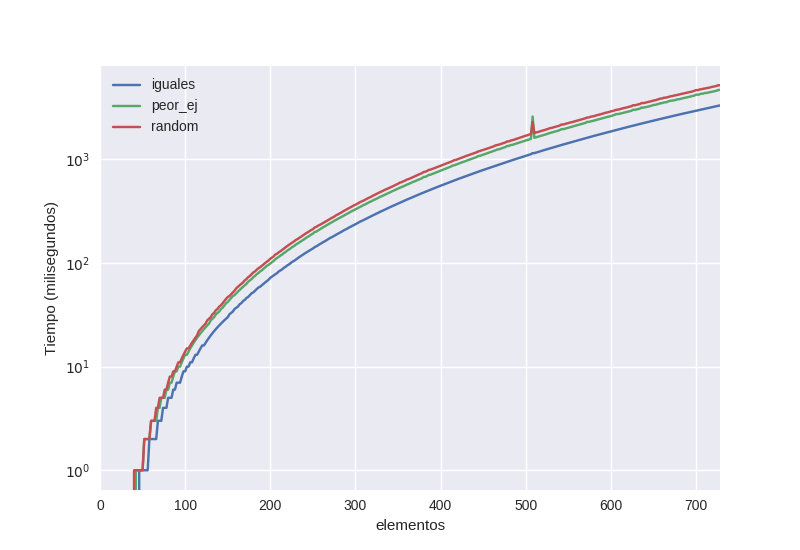
\includegraphics[width=0.55\textwidth]{comp_3_ej3.png}
    \caption{Complejidad temporal}
    \label{fig:mesh1}
\end{figure}

La figura \texttt{5} no muestra demasiada diferencia entre estas curvas, esto sucede porque el tiempo de cómputo requerido para este algoritmo dinámico
se mantiene relativamente constante a la complejidad que es polinomial cúbica

\subsubsection {experimento 2}
Para demostrar que tiene como complejidad polinomial, lo que vamos a hacer es comparar los resultados de alguna de las secuencias contra una
secuencia que representa una función exponencial y otra polinomial y veremos cual es la mejor de estas.
\begin{figure}[h]
    \centering
    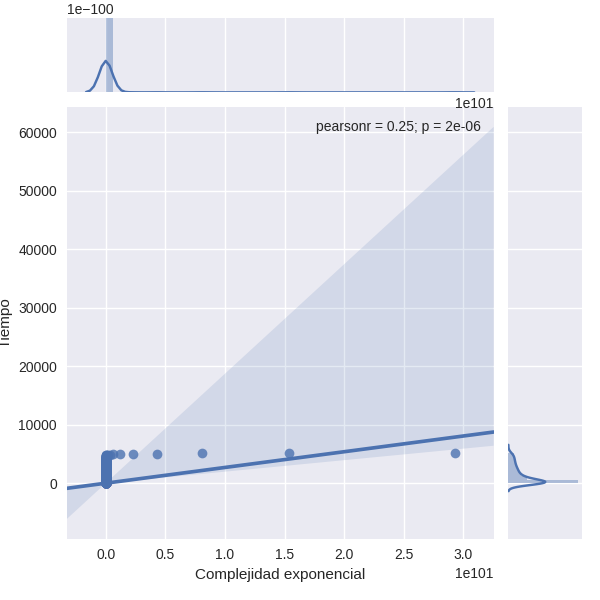
\includegraphics[width=0.38\textwidth]{pearson_ej3_exp.png}
    \caption{Correlación}
    \label{fig:mesh1}
\end{figure}

\begin{figure}[h]
    \centering
    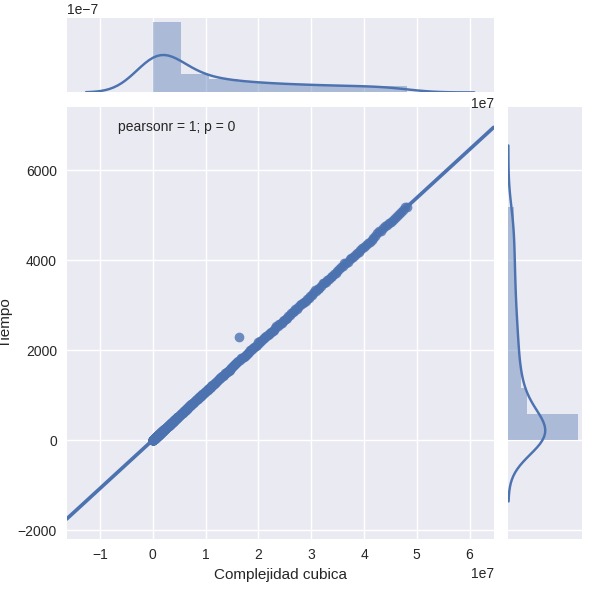
\includegraphics[width=0.38\textwidth]{pearson_ej3_cubico.png}
    \caption{Correlación}
    \label{fig:mesh1}
\end{figure}

La correlación de pearson con una función cúbica es de exactamente 1 contra 0,42 de una función exponencial \texttt{ver figura 6 y 7} . Lo cual implica que
la complejidad es polinomial cúbica.
